\documentclass[runningheads]{llncs}

\usepackage{amsmath,amssymb,amsfonts}
\usepackage{graphicx}
\usepackage{tikz}
\usetikzlibrary{arrows.meta,shapes.geometric,positioning,fit,backgrounds,patterns}
\usepackage{booktabs}
\graphicspath{{figures/}}
\usepackage[protrusion=false,expansion=false]{microtype}
\usepackage{xcolor}
\usepackage[hidelinks]{hyperref}

\begin{document}

\title{Modeling Authorization Saturation in AI-Governed Institutions}
\titlerunning{Modeling Authorization Saturation in AI-Governed Institutions}

\author{Shauray Gupta\inst{1}}
\authorrunning{S. Gupta}

\institute{SM Shetty International School, Mumbai, India\\
\email{shauray.gupta@smshettyinternational.edu}}

\maketitle

\begin{abstract}
Institutions deploying AI decision-support systems face a capacity mismatch that
governance frameworks have not formalized: AI reduces the marginal cost of generating
decision recommendations toward zero, but the cost of authorizing each recommendation---%
human review, contestation, accountability assignment---remains fixed at reviewer
capacity. We model this authorization-production asymmetry as a two-stage queueing model:
a non-bottlenecked production stage (AI throughput) feeds an authorization stage (human
review capacity) with state-dependent service rates. Reviewers exhibit threshold-switching:
when queue length exceeds a tolerance threshold, service transitions from
substantive ($\mu_s$) to ceremonial mode ($\mu_c = \alpha\mu_s$, $\alpha > 1$), trading
quality for throughput. We derive the steady-state authorization quality function
$\bar{Q}(\rho_s)$ and show it undergoes an inflection at a critical utilization
threshold $\rho^* = k/(1+k)$, where $k$ is the institutional tolerance multiplier,
above which quality decline steepens.
Simulation reproduces the transition and reveals that capacity investment is more
effective than throughput regulation below $\rho^*$, while above it neither
intervention alone can restore substantive review. We identify four policy levers
and their effectiveness regions, providing a formal computational
basis for analyzing \emph{authorization saturation} in AI-governed institutions.
\end{abstract}

\keywords{authorization saturation \and queueing theory \and AI governance \and
behavioral tipping points \and computational social science \and ceremonial review}

\section{Introduction}
\label{sec:intro}

When the Dutch Tax and Customs Administration deployed a self-learning algorithm
to flag childcare benefit fraud, human reviewers processed the resulting referrals
at speed: 26,000 families were falsely accused, benefits were halted without
meaningful individual review, and the resulting scandal brought down the
government in 2021~\cite{amnesty2021}. The reviewers were not negligent---they
were saturated. The algorithm generated fraud referrals faster than the review
infrastructure could substantively process them, and the institution adapted by
accelerating review rather than throttling intake. The same structural pattern
recurs across institutions deploying AI decision support: formal oversight
requirements are satisfied on paper while substantive human judgment is
progressively hollowed out in practice. Clinicians sign off on AI-flagged
diagnoses without reviewing the evidence. Benefits officers approve algorithmic
determinations within the allotted review window. Compliance officers certify AI
outputs against checklists without reconstructing the reasoning behind
them~\cite{green2022,elish2019}.

Existing explanations reach for individual cognition---alert fatigue~\cite{parasuraman1997},
automation bias~\cite{bainbridge1983}---or institutional culture~\cite{power1997}. These
accounts are incomplete: the failure pattern recurs across institutions with
different cultures and reviewer attentiveness levels, pointing toward a structural
driver. The U.S. Veterans Benefits Administration, for instance, saw its claims
backlog balloon from 175,000 to over 400,000 after the 2022 PACT Act expanded
eligibility~\cite{va2024}: AI-assisted claim triage accelerated intake while
adjudicator capacity remained fixed, producing the
authorization-production asymmetry our model captures.

The asymmetry is sharpest where AI systems issue recommendations faster
than review processes were designed to absorb. The \emph{production process} generates
outputs at near-zero marginal cost; the \emph{authorization process} does not scale:
every recommendation requires a human reviewer bounded by count, attention, and
procedural infrastructure~\cite{luhmann1969,bovens2007}.

As the authorization queue fills beyond substantive capacity, review becomes
\emph{ceremonial}: form persists while substance does
not~\cite{meyer1977,power1997}.
Administrative burden research documents this: processing rates hold while
time-per-case collapses~\cite{herd2018}.

We synthesize behavioral queueing~\cite{delasay2016,kcterwiesch2009},
institutional theory~\cite{meyer1977}, and administrative burden~\cite{herd2018}
into a compact queueing framework for AI-governed authorization systems
(\S\ref{sec:model}), derive a closed-form saturation threshold
$\rho^* = k/(1+k)$ where $k$ is the institutional tolerance multiplier
(\S\ref{sec:analysis}), map four governance interventions to their effectiveness
regions (\S\ref{sec:interventions}), and reproduce the threshold via discrete-event
simulation (\S\ref{sec:simulation}).

While the queueing machinery is standard, its institutional interpretation is not:
the parameter $k$ bridges organizational theory and queueing dynamics, yielding a
threshold computable from observable indicators and intervention rankings that differ
from common policy intuition.

\section{Related Work}
\label{sec:related}

Green~\cite{green2022} documents that oversight mandates for government AI systems
confer legitimacy without conferring capacity. Elish~\cite{elish2019} traces how
formal accountability concentrates on humans positioned too downstream to exercise
genuine oversight (``moral crumple zones''). Neither paper identifies the
structural conditions that generate these patterns or the operating threshold at
which they become predictable.

Deskilling~\cite{bainbridge1983}, automation bias~\cite{parasuraman1997}, and alert
fatigue~\cite{ancker2017} are individual-level cognitive accounts. Authorization
saturation operates at the institutional level: it occurs even when every reviewer
is capable and attentive, once the procedural infrastructure cannot process
substantive requests at the required throughput.

\noindent\textbf{Institutional ceremony and decoupling.}
Meyer and Rowan~\cite{meyer1977} showed that organizations decouple formal structures
from technical practice under institutional pressure; Power~\cite{power1997}
documented the same substitution in audit practice. Luhmann~\cite{luhmann1969}
grounds decision legitimacy in procedural participation. Here the driver differs:
decoupling is mechanically induced when throughput exceeds authorization capacity.

\noindent\textbf{Behavioral queueing and load effects.}
Delasay et al.~\cite{delasay2016} model state-dependent service rates where servers
adapt to load---a more general framework than our binary switching. KC and
Terwiesch~\cite{kcterwiesch2009} empirically show workload increases speed while
reducing quality. These models treat the switching threshold as exogenous; they
do not parameterize it as institutional tolerance, derive a closed-form
saturation threshold, or map variables to observable governance indicators.
Our model is a special case of Delasay et al.; our contribution is the
institutional interpretation and operationalization. Queueing
theory~\cite{kleinrock1975} provides the formal
apparatus; Herd and Moynihan~\cite{herd2018} treat administrative burden as a
structural capacity constraint.

\noindent\textbf{AI governance and capacity.}
Coglianese and Lehr~\cite{coglianese2017} show that regulatory throughput---not
model accuracy---is the binding governance constraint. Veale et al.~\cite{veale2018}
document chronically under-resourced human review. Selbst et al.~\cite{selbst2019}
and Raji et al.~\cite{raji2020} address fairness and auditing but not capacity
constraints. We formalize these observations with the queueing apparatus above.

\section{Model}
\label{sec:model}

\subsection{System Description}

The system comprises two stages (Fig.~\ref{fig:architecture}).
External decisions arrive at rate $\Lambda$ (Poisson). The \emph{production process}
serves these with the AI system at rate $\mu_p \gg \Lambda$, making it effectively
non-bottlenecked; the effective output is $\lambda \approx \Lambda$.

The \emph{authorization process} is the bottleneck. Premises arrive at rate
$\lambda$. There are $c$ human reviewers with threshold-dependent service:
when the queue is short, review is substantive; when it grows long, reviewers
switch to ceremonial mode (rapid sign-off)---a satisficing response to queue
pressure~\cite{simon1947}. The parameter $k$ encodes
institutional tolerance before heuristic processing replaces deliberation;
we interpret $k$ as a governance parameter measurable from override rates and
review-time distributions, distinguishing it from the exogenous thresholds
in prior behavioral queueing models~\cite{delasay2016,kcterwiesch2009}.

\begin{figure}[t]
\centering
\resizebox{\linewidth}{!}{%
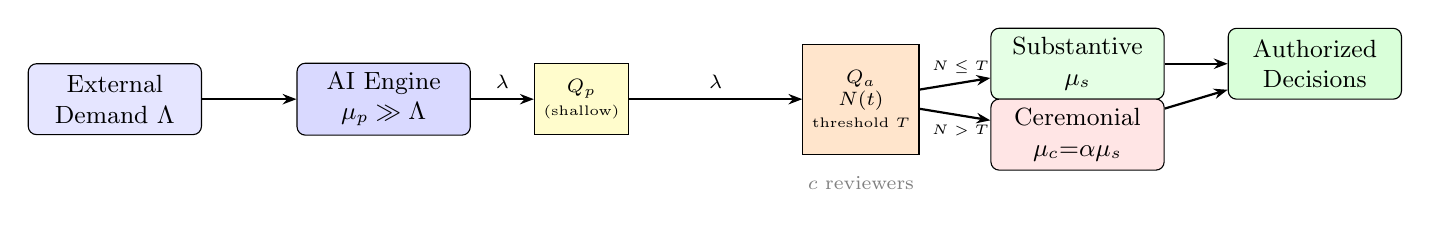
\begin{tikzpicture}[
  box/.style={draw, rounded corners=3pt, minimum width=2.2cm, minimum height=0.9cm,
              align=center, font=\small},
  queue/.style={draw, minimum width=1.0cm, minimum height=0.9cm, align=center, font=\scriptsize},
  arr/.style={-{Stealth[length=5pt]}, thick},
  node distance=0.5cm
]
\node[box, fill=blue!10] (demand) {External\\Demand $\Lambda$};
\node[box, fill=blue!15, right=1.2cm of demand] (ai) {AI Engine\\$\mu_p \gg \Lambda$};
\node[queue, right=0.8cm of ai, fill=yellow!20] (pq) {$Q_p$\\\tiny(shallow)};
\node[queue, right=2.2cm of pq, fill=orange!20, minimum height=1.4cm] (aq) {$Q_a$\\$N(t)$\\\tiny threshold $T$};
\node[box, right=0.9cm of aq, fill=green!10, minimum height=0.7cm, yshift=0.45cm] (sub) {Substantive\\$\mu_s$};
\node[box, right=0.9cm of aq, fill=red!10, minimum height=0.7cm, yshift=-0.45cm] (cer) {Ceremonial\\$\mu_c{=}\alpha\mu_s$};
\node[box, right=0.8cm of sub, fill=green!15] (auth) {Authorized\\Decisions};

\draw[arr] (demand) -- (ai);
\draw[arr] (ai) -- node[above, font=\scriptsize] {$\lambda$} (pq);
\draw[arr] (pq) -- node[above, font=\scriptsize] {$\lambda$} (aq);
\draw[arr] (aq) -- node[above, font=\tiny, xshift=2pt] {$N\leq T$} (sub);
\draw[arr] (aq) -- node[below, font=\tiny, xshift=2pt] {$N>T$} (cer);
\draw[arr] (sub) -- (auth);
\draw[arr] (cer) -- node[below right, font=\scriptsize] {} (auth);

\node[below=0.15cm of aq, font=\scriptsize, text=gray] {$c$ reviewers};
\end{tikzpicture}%
}% end resizebox
\caption{Coupled two-queue system. The production queue $Q_p$ (AI engine) is
never bottlenecked; the authorization queue $Q_a$ is the binding constraint.
When queue length $N(t)$ exceeds threshold $T = kc$, reviewers switch from
substantive ($\mu_s$) to ceremonial mode ($\mu_c = \alpha\mu_s$, $\alpha > 1$).}
\label{fig:architecture}
\end{figure}

\subsection{Formal Queueing Model}

We model the authorization queue as an $M/M/c$ queue with state-dependent service rates.
Let $N(t)$ denote the number of authorizations pending or in service at time $t$.
The queue has Poisson arrivals at rate $\lambda$, $c$ servers, and a tolerance
threshold $T = kc$ for integer $k \geq 1$.

\medskip
\noindent\textbf{State-dependent service rates.} The per-server rate is:
\begin{equation}
\mu(n) = \begin{cases}
\mu_s & \text{if } n \leq T \\
\mu_c = \alpha\mu_s & \text{if } n > T
\end{cases}
\label{eq:service-rate}
\end{equation}
where $\alpha > 1$ reflects that ceremonial review is faster (but lower quality)
than substantive review. The total service rate when $n$ authorizations are in the
system is $\nu(n) = \min(n, c) \cdot \mu(n)$.

\medskip
\noindent\textbf{Authorization quality.} Each authorization has quality
$q(n) \in [q_c, q_s]$ where $q_s = 1$ (fully substantive) and
$0 < q_c < q_s$ (ceremonial quality):
\begin{equation}
q(n) = \begin{cases}
q_s & \text{if } n \leq T \\
q_c & \text{if } n > T
\end{cases}
\label{eq:quality}
\end{equation}

\subsection{Steady-State Analysis}

Since $N(t)$ is a birth-death process with birth rate $\lambda$ and state-dependent
death rates $\nu(n)$, the steady-state distribution satisfies the detailed balance
equations. Let $\rho_s = \lambda/(c\mu_s)$ denote the substantive utilization ratio
and $\rho_c = \lambda/(c\mu_c) = \rho_s/\alpha$ the ceremonial utilization ratio.
For stability we require $\rho_c < 1$, i.e., $\rho_s < \alpha$.

The stationary probabilities $\{\pi_n\}$ are:
\begin{equation}
\pi_n = \pi_0 \cdot A_n, \quad
A_n = \frac{\lambda^n}{\prod_{i=1}^{n} \nu(i)}
\label{eq:stationary}
\end{equation}

Explicitly:
\begin{align}
A_n &= \frac{(c\rho_s)^n}{n!}, \quad 0 \leq n \leq c \label{eq:An-low}\\
A_n &= \frac{(c\rho_s)^c}{c!} \cdot \rho_s^{n-c}, \quad c < n \leq T \label{eq:An-mid}\\
A_n &= A_T \cdot \rho_c^{n-T}, \quad n > T \label{eq:An-high}
\end{align}

The last set forms a geometric series. The normalization constant satisfies:
\begin{equation}
\pi_0^{-1} = \sum_{n=0}^{c} \frac{(c\rho_s)^n}{n!}
  + \frac{(c\rho_s)^c}{c!} \cdot \frac{\rho_s(1-\rho_s^{T-c})}{1-\rho_s}
  + A_T \cdot \frac{\rho_c}{1-\rho_c}
\label{eq:normalization}
\end{equation}
(The middle term has the limiting form $(T{-}c)(c\rho_s)^c/c!$ as $\rho_s\to 1$
by L'H\^opital's rule; the tail converges for $\rho_c = \rho_s/\alpha < 1$.)

The mean steady-state authorization quality is:
\begin{equation}
\bar{Q}(\rho_s) = q_s\, P(N \leq T) + q_c\, P(N > T)
= q_s - (q_s - q_c)\, P(N > T)
\label{eq:quality-mean}
\end{equation}

where $P(N > T) = \pi_0 \cdot A_T \cdot \rho_c/(1-\rho_c)$.

\section{Analysis}
\label{sec:analysis}

\subsection{The Saturation Threshold}

We characterize the utilization level $\rho^*$ at which the system transitions
from predominantly substantive to predominantly ceremonial review.

\begin{proposition}[Authorization Saturation Threshold]
\label{thm:threshold}
Under the Halfin--Whitt heavy-traffic regime~\cite{halfin1981} (large $c$), the
mean queue length concentrates near $c\rho_s/(1-\rho_s)$. Setting this equal
to the behavioral threshold $T = kc$ gives the saturation threshold:
\begin{equation}
\rho^* \approx \frac{k}{1+k}
\label{eq:threshold}
\end{equation}
\end{proposition}

\noindent\textit{Derivation.}
Setting $c\rho^*/(1-\rho^*) = kc$ and solving yields $\rho^* = k/(1+k)$;
concentration sharpens as $O(c^{-1/2})$ under the Halfin-Whitt regime~\cite{halfin1981}.

\noindent\textit{Approximation note.} The binary switching is an analytically tractable
first-order approximation. A continuous sigmoid transition
$\mu(n) = \mu_s + (\mu_c - \mu_s)\cdot\sigma((n{-}T)/\delta)$ yields
qualitatively identical inflection with the transition broadening proportionally
to $\delta$; the binary model is the limit $\delta \to 0$.
Alert-fatigue studies document threshold-like behavioral transitions~\cite{ancker2017}.

\smallskip\noindent\textit{Sensitivity to switching assumption.}
Simulating with a sigmoid service rate for
$\delta \in \{1, 2, 5\}$, the inflection in $\bar{Q}(\rho_s)$ persists:
at $\delta=1$ the quality drop from $\rho_s=0.4$ to $\rho_s=0.9$ is
11.5\% (vs.\ 17.8\% for binary); at $\delta=5$ it is 4.8\%.
The threshold result is robust; only its sharpness depends on $\delta$.

\noindent Properties of Eq.~(\ref{eq:threshold}):
(i) $\rho^*$ depends only on $k$---not on $\lambda$, $\mu_s$, or $c$ individually;
(ii) $\rho^*$ is increasing in $k$: more tolerant institutions sustain substantive
review longer; (iii) for $k \to \infty$, $\rho^* \to 1$---the standard M/M/c
stability boundary; (iv) for $k = 1$, $\rho^* = 0.5$.

\begin{table}[t]
\centering
\caption{Authorization saturation thresholds $\rho^*$ as a function of
institutional tolerance $k$. Low-$k$ institutions saturate well below nominal capacity.}
\label{tab:thresholds}
\begin{tabular}{@{}lcccccc@{}}
\toprule
$k$ (tolerance) & 0.25 & 0.5 & 1.0 & 2.0 & 3.0 & 5.0 \\
\midrule
$\rho^*$ & 0.20 & 0.33 & 0.50 & 0.67 & 0.75 & 0.83 \\
\bottomrule
\end{tabular}
\end{table}

\subsection{Authorization Quality Function}

Fig.~\ref{fig:quality} plots $\bar{Q}(\rho_s)$ from discrete-event simulation
for three values of $k$ (50 runs per point; 95\% CI bands shown). In each case
the quality function is approximately flat at $q_s$ for $\rho_s < \rho^*$,
declines rapidly near $\rho^*$, and asymptotes toward $q_c$ above it.
The transition sharpens with increasing $c$ (a concentration effect).

\begin{figure}[t]
\centering
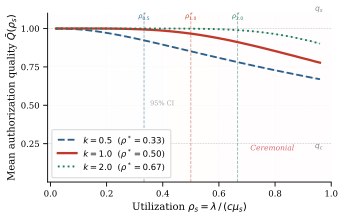
\includegraphics[width=\linewidth]{fig2_quality}
\caption{Mean authorization quality $\bar{Q}(\rho_s)$ for three institutional tolerance
levels $k$ ($c=5$, $\alpha=3$, $q_s=1.0$, $q_c=0.25$). Curves are Monte Carlo means
(50 runs per point, 95\% CI as shaded bands). Dashed verticals mark $\rho^* \approx k/(1+k)$~\cite{halfin1981};
quality decline accelerates at each threshold.}
\label{fig:quality}
\end{figure}

\subsection{Intervention Analysis}
\label{sec:interventions}

We analyze four governance interventions and their effectiveness regions.

\smallskip\noindent\textbf{I1: Capacity investment} ($c \to \beta c$, $\beta > 1$).
Reduces $\rho_s$ to $\rho_s/\beta$ but leaves $\rho^*$ unchanged: delays saturation without preventing it.

\smallskip\noindent\textbf{I2: Throughput regulation} ($\lambda \to \gamma\lambda$, $\gamma < 1$).
Reduces $\rho_s$ directly. Effective below $\rho^*$; above it requires $\gamma < \rho^*/\rho_s$, which may be infeasible.

\smallskip\noindent\textbf{I3: Threshold adjustment} ($k \to k' > k$).
Shifts $\rho^* \to k'/(1+k')$. The most structurally targeted intervention but requires sustained organizational commitment.

\smallskip\noindent\textbf{I4: Ceremonial quality improvement} ($q_c \to q_c' > q_c$).
Reduces the quality drop without shifting the tipping point. Limits damage when I1--I3 are infeasible.

Fig.~\ref{fig:interventions} summarizes the operating regions of each intervention.

\begin{figure}[t]
\centering
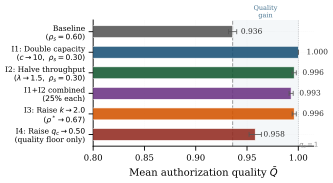
\includegraphics[width=\linewidth]{fig3_interventions}
\caption{Simulation-validated intervention comparison at baseline
$\rho_s = 0.60$ ($\bar{Q}_{\text{base}} = 0.936$, ceremonial fraction $8.5\%$).
I1--I3 (structural) restore near-full quality by addressing $c$, $\lambda$, or $k$;
I4 raises the quality floor without shifting the tipping point.}
\label{fig:interventions}
\end{figure}

\section{Simulation}
\label{sec:simulation}

\subsection{Experimental Setup}

We implement a discrete-event simulation of the state-dependent $M/M/c$ queue
using the standard next-event scheduling algorithm. Service times are drawn
from exponential distributions with rates from Eq.~(\ref{eq:service-rate});
service rate is fixed at job-start (based on $N$ at that moment), and authorization
quality follows Eq.~(\ref{eq:quality}) evaluated at the same instant.

\smallskip\noindent\textbf{Parameters.}
$c = 5$; $\mu_s = 1.0$; $\alpha = 3.0$; $k = 1.0$ ($T = 5$); $q_s = 1.0$, $q_c = 0.25$.
$\lambda$ varies across $\rho_s \in \{0.1, \ldots, 0.9\}$. Each run: $T_{\mathrm{sim}} = 50{,}000$
after $5{,}000$ warm-up. Monte Carlo (50 seeds, $k\in\{0.5,1.0,2.0\}$) confirms
robustness; 95\% CIs in Fig.~\ref{fig:quality}.

\subsection{Results}

\begin{table}[t]
\centering
\caption{Simulation results: $\bar{Q}(\rho_s)$ and $\bar{N}$ across utilization levels
($c=5$, $k=1$, $\alpha=3$). Theoretical $\rho^* = 0.50$.}
\label{tab:simulation}
\begin{tabular}{@{}ccccc@{}}
\toprule
$\rho_s$ & $\lambda$ & $\bar{N}$ (sim.) & $\bar{Q}$ (sim.) & Regime \\
\midrule
0.10 & 0.50 & 0.50  & 1.000 & Substantive \\
0.30 & 1.50 & 1.49  & 0.996 & Substantive \\
0.50 & 2.50 & 2.49  & 0.967 & Transition \\
0.60 & 3.00 & 2.99  & 0.936 & Ceremonial onset \\
0.70 & 3.50 & 3.45  & 0.898 & Ceremonial \\
0.90 & 4.50 & 4.31  & 0.809 & Ceremonial \\
\bottomrule
\end{tabular}
\end{table}

Table~\ref{tab:simulation} reports results. Quality is approximately flat at $q_s$
for $\rho_s < \rho^*$, declines rapidly near $\rho^*$, and asymptotes toward $q_c$.
At $\rho_s = 0.90$, $\bar{Q} = 0.809$ implies $P(N > T) \approx 0.254$:
one in four authorizations is ceremonial.
The ceremonial speedup ($\alpha=3$) maintains queue stability for all
$\rho_s < \alpha = 3.0$---the institution does not fail; it \emph{adapts badly}.

\noindent\textit{Note.} The simulation validates threshold consistency against
the model it implements; empirical operationalization follows below.

\noindent\textbf{Intervention validation.}
At $\rho_s = 0.60$ (baseline $\bar{Q} = 0.936$): doubling capacity ($c \to 10$) restores
$\bar{Q} = 1.000$; halving throughput ($\lambda \to 1.5$) achieves $\bar{Q} = 0.996$;
I1+I2 combined achieves $\bar{Q} = 0.993$; raising $k \to 2.0$ achieves
$\bar{Q} = 0.996$; raising $q_c \to 0.50$ achieves $\bar{Q} = 0.958$.

\subsection{Empirical Operationalization}
\label{sec:empirical}

The model variables map to observable indicators.
Table~\ref{tab:operationalization} applies this mapping to the VBA~\cite{va2024}.

\begin{table}[t]
\centering
\caption{Variable-to-observable mapping for the VBA. $\rho_s > 1$ indicates overload.}
\label{tab:operationalization}
\begin{tabular}{@{}lll@{}}
\toprule
Variable & Observable & VBA estimate \\
\midrule
$\lambda$ & Claims received/year & $\approx$2.5M \\
$c$ & Adjudicator FTE & $\approx$5,000 \\
$\mu_s$ & Claims/FTE/year (low backlog) & $\approx$375 \\
$\rho_s$ & $\lambda/(c\mu_s)$ & $\approx$1.3 \\
$T$ & Backlog threshold (days) & 125 \\
$q_c$ & Appeal reversal rate & 10--15\% \\
\bottomrule
\end{tabular}
\end{table}

The VBA's $\rho_s \approx 1.3$ places it well above $\rho^*$ for any plausible
$k$. The observable signatures are consistent with the model:
mandatory overtime (I1), a 125-day
backlog threshold (operational $T$), and elevated appeal reversal rates
(observable $q_c$). The VBA reinstated mandatory overtime in 2025---a capacity
intervention that reduces $\rho_s$ without shifting $\rho^*$, consistent with
the model's prediction that I1 delays but cannot prevent saturation.

\section{Policy Implications}
\label{sec:policy}

Three findings bear on governance design.

\smallskip\noindent\textbf{P1: Adding reviewers does not raise the saturation threshold.}
$\rho^* = k/(1+k)$ depends on $k$ alone; scaling $c$ reduces $\rho_s$ but leaves
$\rho^*$ fixed if workflow norms are unchanged. Governance frameworks~\cite{euaiact2024,nist2023}
must specify $k$---minimum review time, contestation requirements---not only $c$.

\smallskip\noindent\textbf{P2: Procurement contracts are the primary intervention window.}
Once $\rho_s > \rho^*$, restoring substantive review requires expensive post-deployment
interventions. Procurement specifications that cap $\lambda$, require minimum review time,
or mandate contestation infrastructure set $\rho_s$ and $k$ before deployment.

\smallskip\noindent\textbf{P3: Reviewer-level interventions do not shift the threshold.}
Training and interface redesign~\cite{parasuraman1997} operate on $q_c$, not $\rho^*$.

\section{Conclusion}
\label{sec:conclusion}

The queueing model is a special case of Delasay et al.~\cite{delasay2016};
our contribution is its institutional interpretation. The key insight is that
$k$ (\S\ref{sec:model})---not headcount---is the primary governance lever:
it is measurable from administrative data, modifiable through procedural
requirements, and yields a threshold $\rho^*$ that capacity investment cannot
shift. Ceremonial review is structurally induced: AI's near-zero marginal
production cost against the fixed cost of human authorization produces the
asymmetry without negligence.

Future work should extend to multi-tier authorization networks (Jackson networks)
and non-exponential service times (GI/GI/c limits~\cite{whitt2002}). Empirical
estimation of $k$ from override rates and review-time distributions, building on
\S\ref{sec:empirical}, is a priority.


\bibliographystyle{splncs04}
\bibliography{references}

\end{document}
